% ----------------------------------------------------------------------------------------
%--- CHAPTER INTRODUCTION ----------------------------------------------------------------
% ----------------------------------------------------------------------------------------
\chapter{Introduction} \label{introduction}

\enquote{\emph{Pantha Rhei}} is, according to \emph{Plato}, one of the famous
philosophical statements first described by the Greek philosopher
\emph{Heraclitus}.\footnote{\url{https://plato.stanford.edu/entries/process-philosophy/}}
Translated as \enquote{everything flows} this statement is an unambiguous commitment to
ubiquitous dynamics of everything that exists. \enquote{Life is flux}, one of the
constants in life is change and its best we act accordingly.

In the realms of Software Engineering the \enquote{laws of software evolution}
\parencite[]{lehman_programs_1980} refers to a series of laws described by
\citeauthor{lehman_programs_1980} starting from 1974. With these Laws, he describes the
balance between the forces driving new developments on the one hand (a change), and the
forces that slow down progress on the other hand. Based on \emph{Heraclitus} philosophical
statement we assume a software engineering project frequently will be subjected to change,
possibly due to changing functional requirements and technological progress. As these
changes emerges, the complexity of these software projects will gradually increase over
time. If the system is not adapted appropriately the combinatorial effects of these
changes will result in ever-increasing complexity and render the software system
eventually obsolete, according to \citeauthor{lehman_programs_1980}
\parencite[]{lehman_programs_1980}.

As the competitive environments of contemporary organizations are changing continuously,
the speed at which changes follow each other is also increasing. IT organization are
attempting to cope with this trend by adopting agility and maturing its agile practices
\parencite[]{2024_SIM_key_issues_and_trends}. Agility is defined as a measure for
contemporary organizations to adept to new environments and to cope with rapid change
\parencite[]{neumann_strategic_1994}.

% ----------------------------------------------------------------------------------------
%--- SECTION INTRODUCING SOFTWARE EVOLVABILITY -------------------------------------------
% ----------------------------------------------------------------------------------------
\section{Introducing Software evolvability}
<<To-do: Link software evolvability to first part of the introduction>>\\
<<To-do: Link combinatorial effects to a measure to determine software evolvability>>

% ----------------------------------------------------------------------------------------
%--- SECTION INTRODUCING NORMALIZED SYSTEMS THEOREMS -------------------------------------
% ----------------------------------------------------------------------------------------
\section{Introducing Normalized Systems Theorems}
<<To-do: Link normalized systems as a measure to create software evolvability>>

% ----------------------------------------------------------------------------------------
%--- SECTION INTRODUCING CLEAN ARCHITECTURE ___-------------------------------------------
% ----------------------------------------------------------------------------------------
\section{Introducing Clean Architecture}
<<To-do: Link normalized systems as a measure to create software evolvability>>

% ----------------------------------------------------------------------------------------
%--- SECTION PROBLEM STATEMENT -----------------------------------------------------------
% ----------------------------------------------------------------------------------------
\section{Problem statement} \label{problem_statement}

Companies applying the Normalized Systems Theory to their products primarily use Java EE,
a programming language. The company NSX
\footnotetext{\url{https://normalizedsystems.org/}} for example, has implemented their
generation tools, modeling suite (Prime Radiant), and expander using this programming
language. Java EE is still a prevalent programming language for enterprise- and IT
organizations. Many software solutions are created and maintained using this programming
language. However, the Normalized Systems theorems are not only applicable to Java EE. The
principles and design patterns derived from the Normalized Systems Theorem apply to any
object-oriented programming language. 

Another example of a popular programming language in enterprise-, and IT organizations is
C\#. There is however no documented research, or proof of experiences on C\# software
projects using Normalized Systems Theory with the aspects of expansion and harvesting \&
rejuvenation.

% ----------------------------------------------------------------------------------------
%--- SECTION HYPOTHESIS -----------------------------------------------------------
% ----------------------------------------------------------------------------------------
\section{Hypothesis} \label{hypothesis}
\begin{figure}[!h]
    \centering
    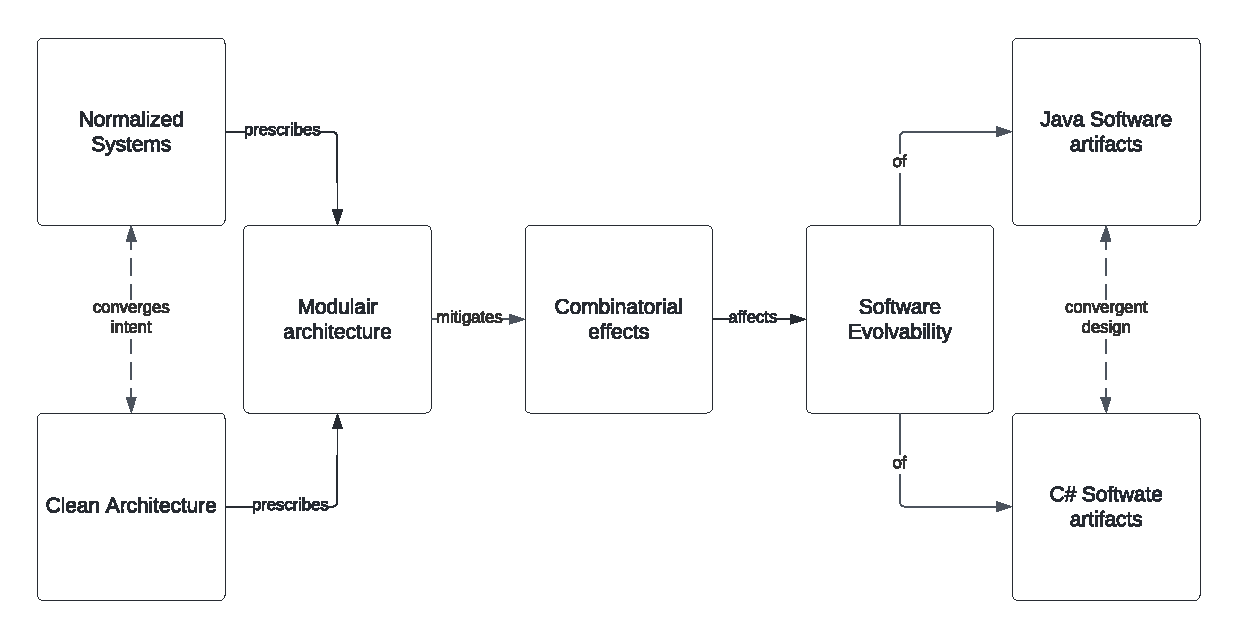
\includegraphics[width=1\textwidth]{Figures/hypothesis.pdf}
    \caption[The hypothesis graphically.]{The hypothesis graphically.}
    \label{fig:hypothesis}
\end{figure}

% ----------------------------------------------------------------------------------------
%--- SECTION RESEARCH SUBJECT -----------------------------------------------------------
% ----------------------------------------------------------------------------------------
\section{Conceptual framework} \label{conceptual_framework}
Figure \ref{fig:overall_conceptual_framework} depicts the conceptual research framework.
It describes the hypothesis that Normalized Systems Theorems have a positive impact on the
total amount of combinatorial effects on C\# based information systems.

\begin{figure}[!h]
    \centering
    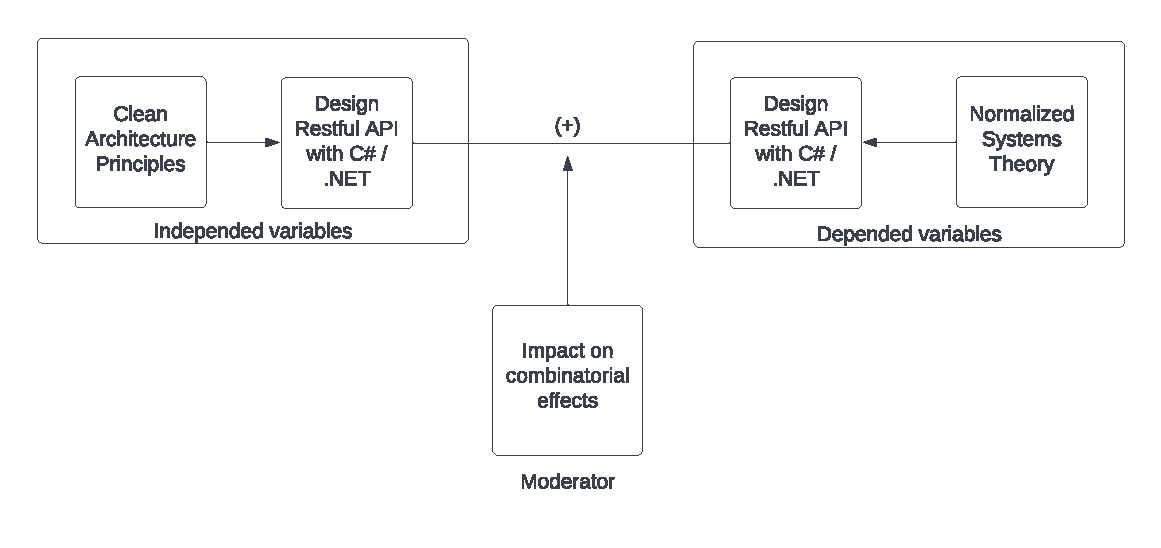
\includegraphics[width=1\textwidth]{Figures/overall_conceptual_framework}
    \caption[Overall conceptual framework]{Overall conceptual framework.}
    \label{fig:overall_conceptual_framework}
\end{figure}
\newpage
% ----------------------------------------------------------------------------------------
%--- SECTION RESEARCH QUESTION -------------------------------------------------------------------
% ----------------------------------------------------------------------------------------
\section{Research questions} \label{research_questions}
Considering the hypothesis described in \ref{conceptual_framework} the following research
is determined:

\begin{center}
    \enquote*{\textit{What is the applicability of Normalized Systems Theorems
    on restful API's designed based on the Clean Architecture principles and build with
    C\#/.NET}}
\end{center}

The following sub-questions can be formulated that support the research on the main
research question:
\begin{itemize}
    \item What is the literature stating about evolvable software systems.
    \item What is the literature stating about combinatorial effects on software changes in software systems.
    \item What is the literature stating on how one can measure combinatorial effects of a change on a software system.
    \item Which principles of Clean Architecture contribute to a reduction of
    combinatorial effects, in a way that they complement the theorems of normalized
    systems.
\end{itemize}